\documentclass[14pt, fleqn, xcolor={dvipsnames, table}]{beamer}
\usepackage[T2A]{fontenc}
\usepackage[utf8]{inputenc}
\usepackage[english,russian]{babel}
\usepackage{amssymb,amsfonts,amsmath,mathtext}
\usepackage{cite,enumerate,float,indentfirst}
\usepackage{cancel}
\usepackage{color}
\usepackage{hyperref}
\hypersetup{colorlinks,urlcolor=NavyBlue}

\usepackage{tikz}                   
\usetikzlibrary{shadows}

% \usepackage{enumitem}
% \setitemize{label=\usebeamerfont*{itemize item}%
%   \usebeamercolor[fg]{itemize item}
%   \usebeamertemplate{itemize item}}

\graphicspath{{images/}}

\usetheme{Boadilla}
\usecolortheme{seahorse}
\usefonttheme{serif}
\renewcommand{\CancelColor}{\color{red}}

\setbeamercolor{footline}{fg=Blue!50}
\setbeamertemplate{footline}{
  \leavevmode%
  \hbox{%
  \begin{beamercolorbox}[wd=.333333\paperwidth,ht=2.25ex,dp=1ex,center]{}%
    Амосов Федор, СПбГУ
  \end{beamercolorbox}%
  \begin{beamercolorbox}[wd=.333333\paperwidth,ht=2.25ex,dp=1ex,center]{}%
    Санкт-Петербург, 2014
  \end{beamercolorbox}%
  \begin{beamercolorbox}[wd=.333333\paperwidth,ht=2.25ex,dp=1ex,right]{}%
  Стр. \insertframenumber{} из \inserttotalframenumber \hspace*{2ex}
  \end{beamercolorbox}}%
  \vskip0pt%
}
\newcommand\indentdisplays[1]{%
     \everydisplay{\addtolength\displayindent{#1}%
     \addtolength\displaywidth{-#1}}}
\newcommand{\itemi}{\item[\checkmark]}

\title{Построение карты пылевых облаков\\\small{}}
\author[]{
    \small{
        Амосов Федор, СПбГУ\\
        ~\\
        Руководитель: Цветков Александр, СПбГУ
    }
}
\date{}

\begin{document}

    \begin{frame}
        \maketitle
        \small
    \end{frame}

    \section{Постановка задачи}  
    
        \begin{frame}{Постановка задачи}
            Дан звездный каталог с данными о
            \begin{itemize}
                \item положениях
                \item параллаксах
                \item фотометрии
                \item спектральных классах и классах светимости
            \end{itemize}  
            Задача
            \begin{itemize}
                \item Построить трехмерную карту пылевых облаков 
            \end{itemize}         
        \end{frame}
        
        \begin{frame}{Локальная задача}
            Дан звездный каталог с данными о
            \begin{itemize}
                \item положениях
                \item параллаксах
                \item фотометрии
                \item спектральных классах и классах светимости
            \end{itemize}  
            Задача
            \begin{itemize}
                \item Построить панораму пылевых облаков
            \end{itemize}         
        \end{frame}
        
        \begin{frame}{Каталог}
            Ззвездный каталог с данными о
            \begin{itemize}
                \item положениях
                \item параллаксах
                \item фотометрии
                \item спектральных классах и классах светимости
            \end{itemize}  
            $\Longrightarrow$ каталог Hipparcos ($10^5$ звезд)
        \end{frame}
        
    \section{Определения}
        \begin{frame}{Покраснение}
            $$
                E_{B - V} = (B - V)_{obs} - (B - V)_{int}
            $$
            Пример на звезде HIP 44800
            \begin{itemize}
                \item У нее в каталоге $(B - V)_{obs} = 0.535^m$
                \item Класс F7V, поэтому $(B - V)_{int} = 0.493^m$
                \item Покраснение $0.535^m - 0.493^m = 0.042^m$
                \item Между нами и звездой пыли на $0.042^m$
            \end{itemize}
        \end{frame}

    \section{Зависимость покраснения от расстояния}    
    
        \begin{frame}{Идеальная кривая покраснения}
            \begin{center}
                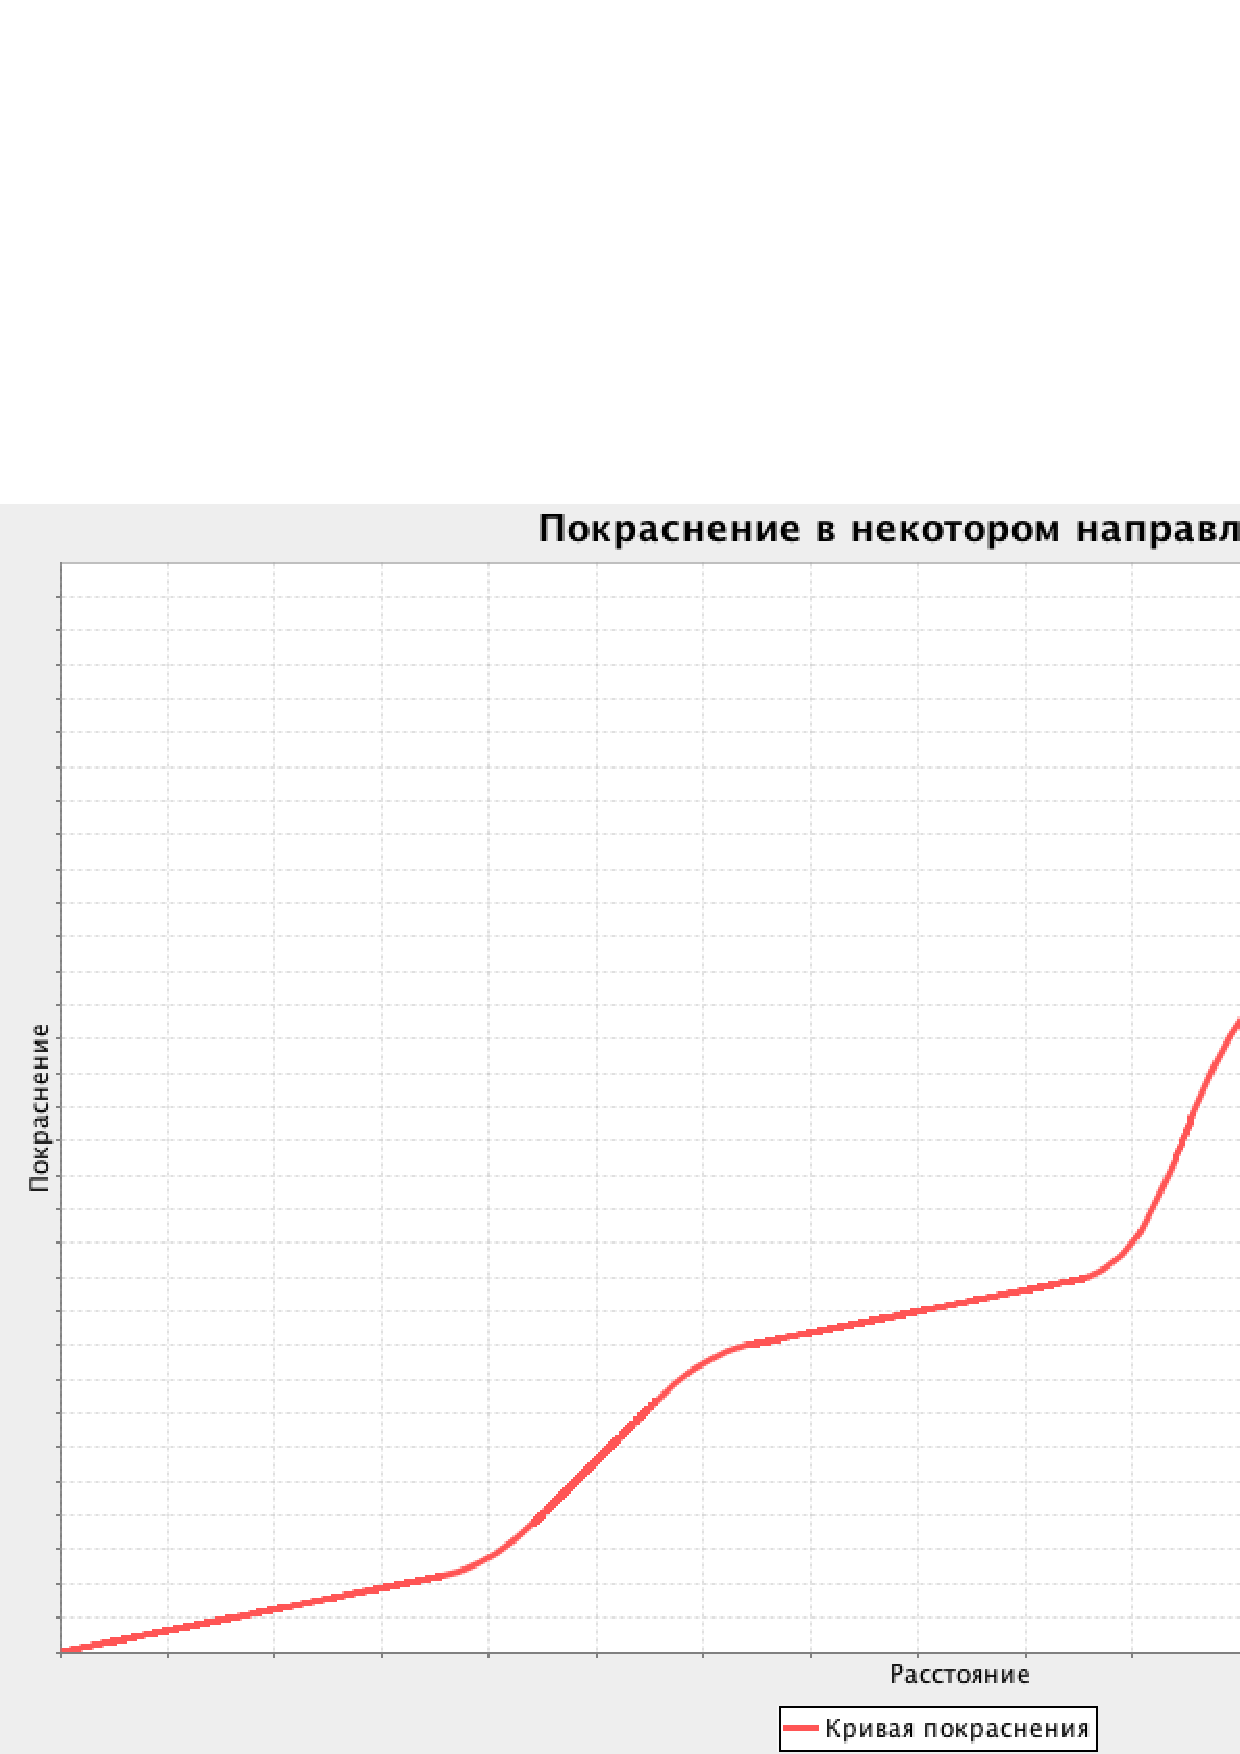
\includegraphics[scale=0.35]{ideal-1-no-tick.png}
            \end{center}             
        \end{frame}
        
        \begin{frame}{Пылевые облака}
            \begin{center}
                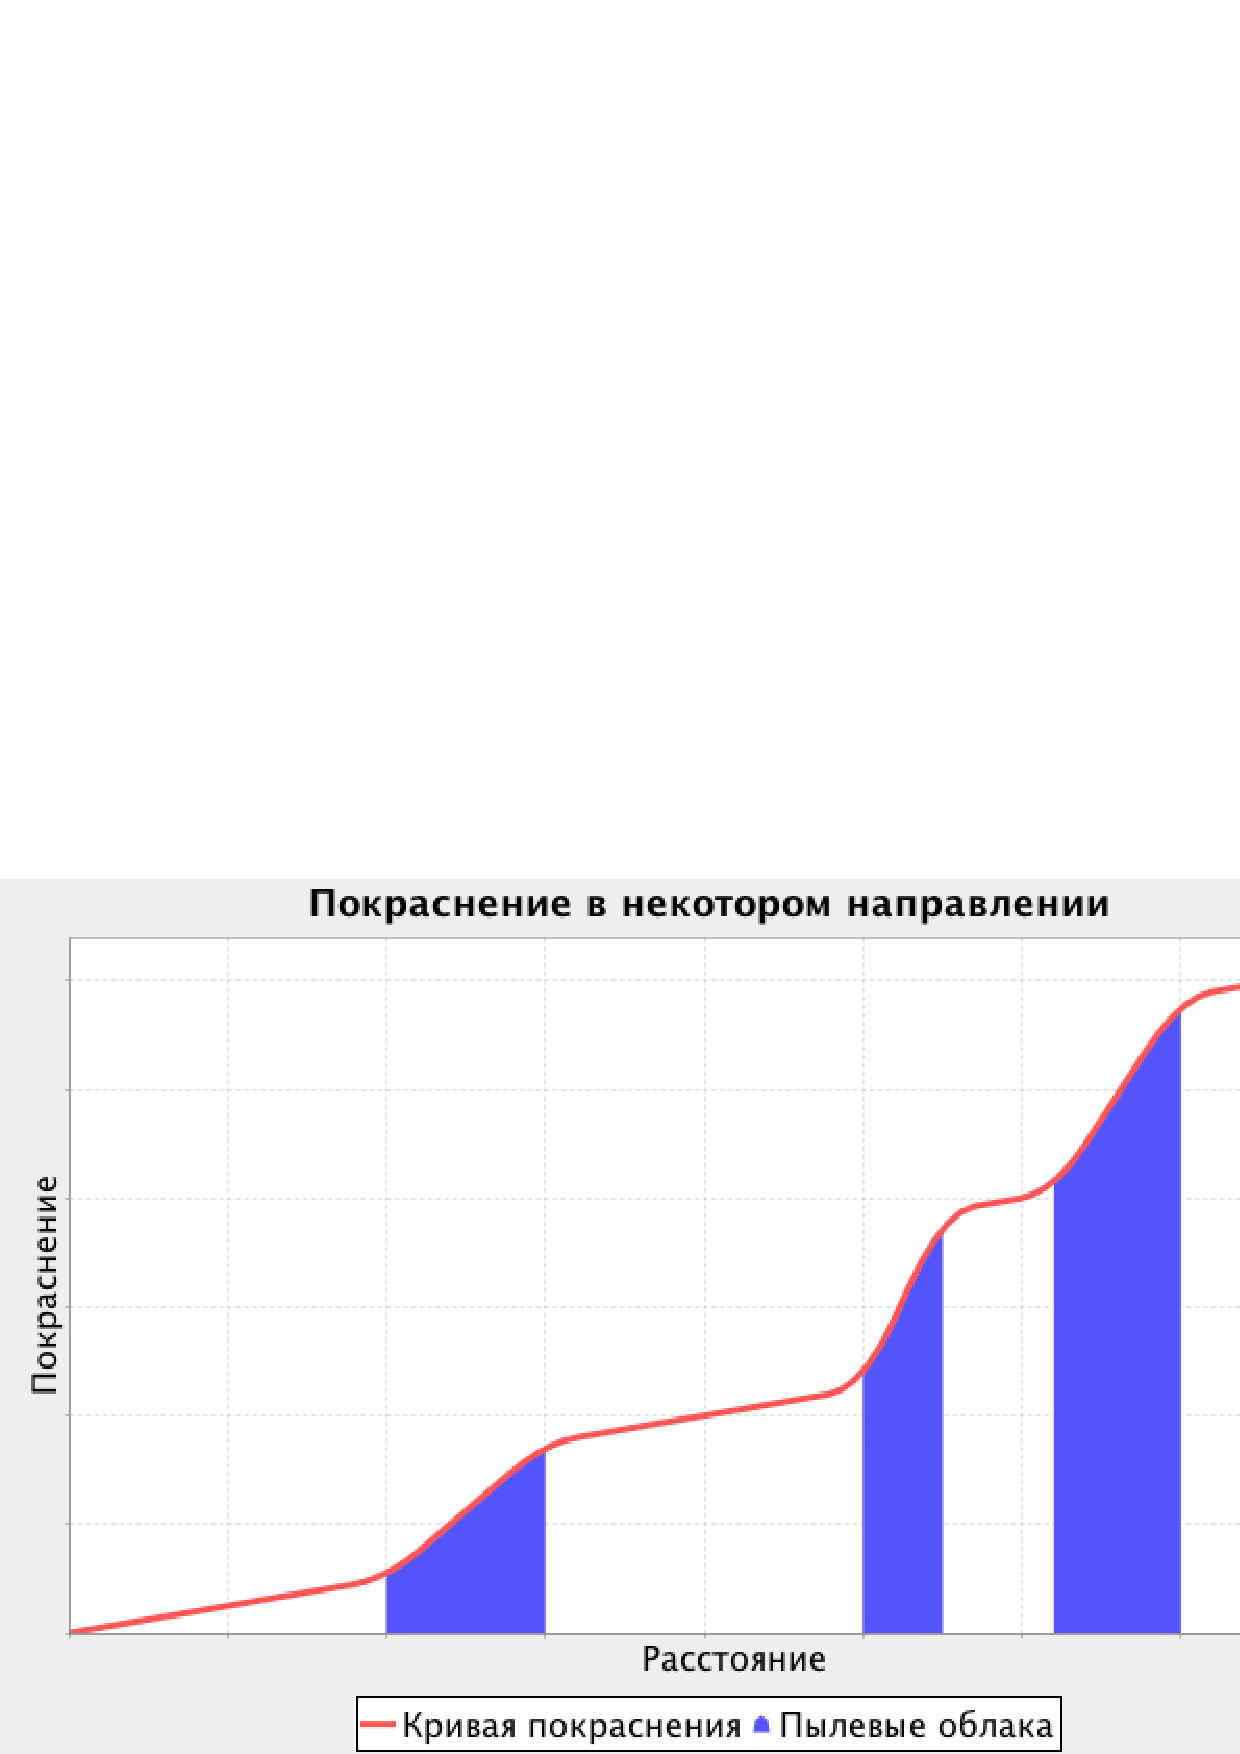
\includegraphics[scale=0.35]{ideal-2-no-tick.png}
            \end{center}             
        \end{frame}
        
        \begin{frame}{Реальное покраснение}
            \begin{center}
                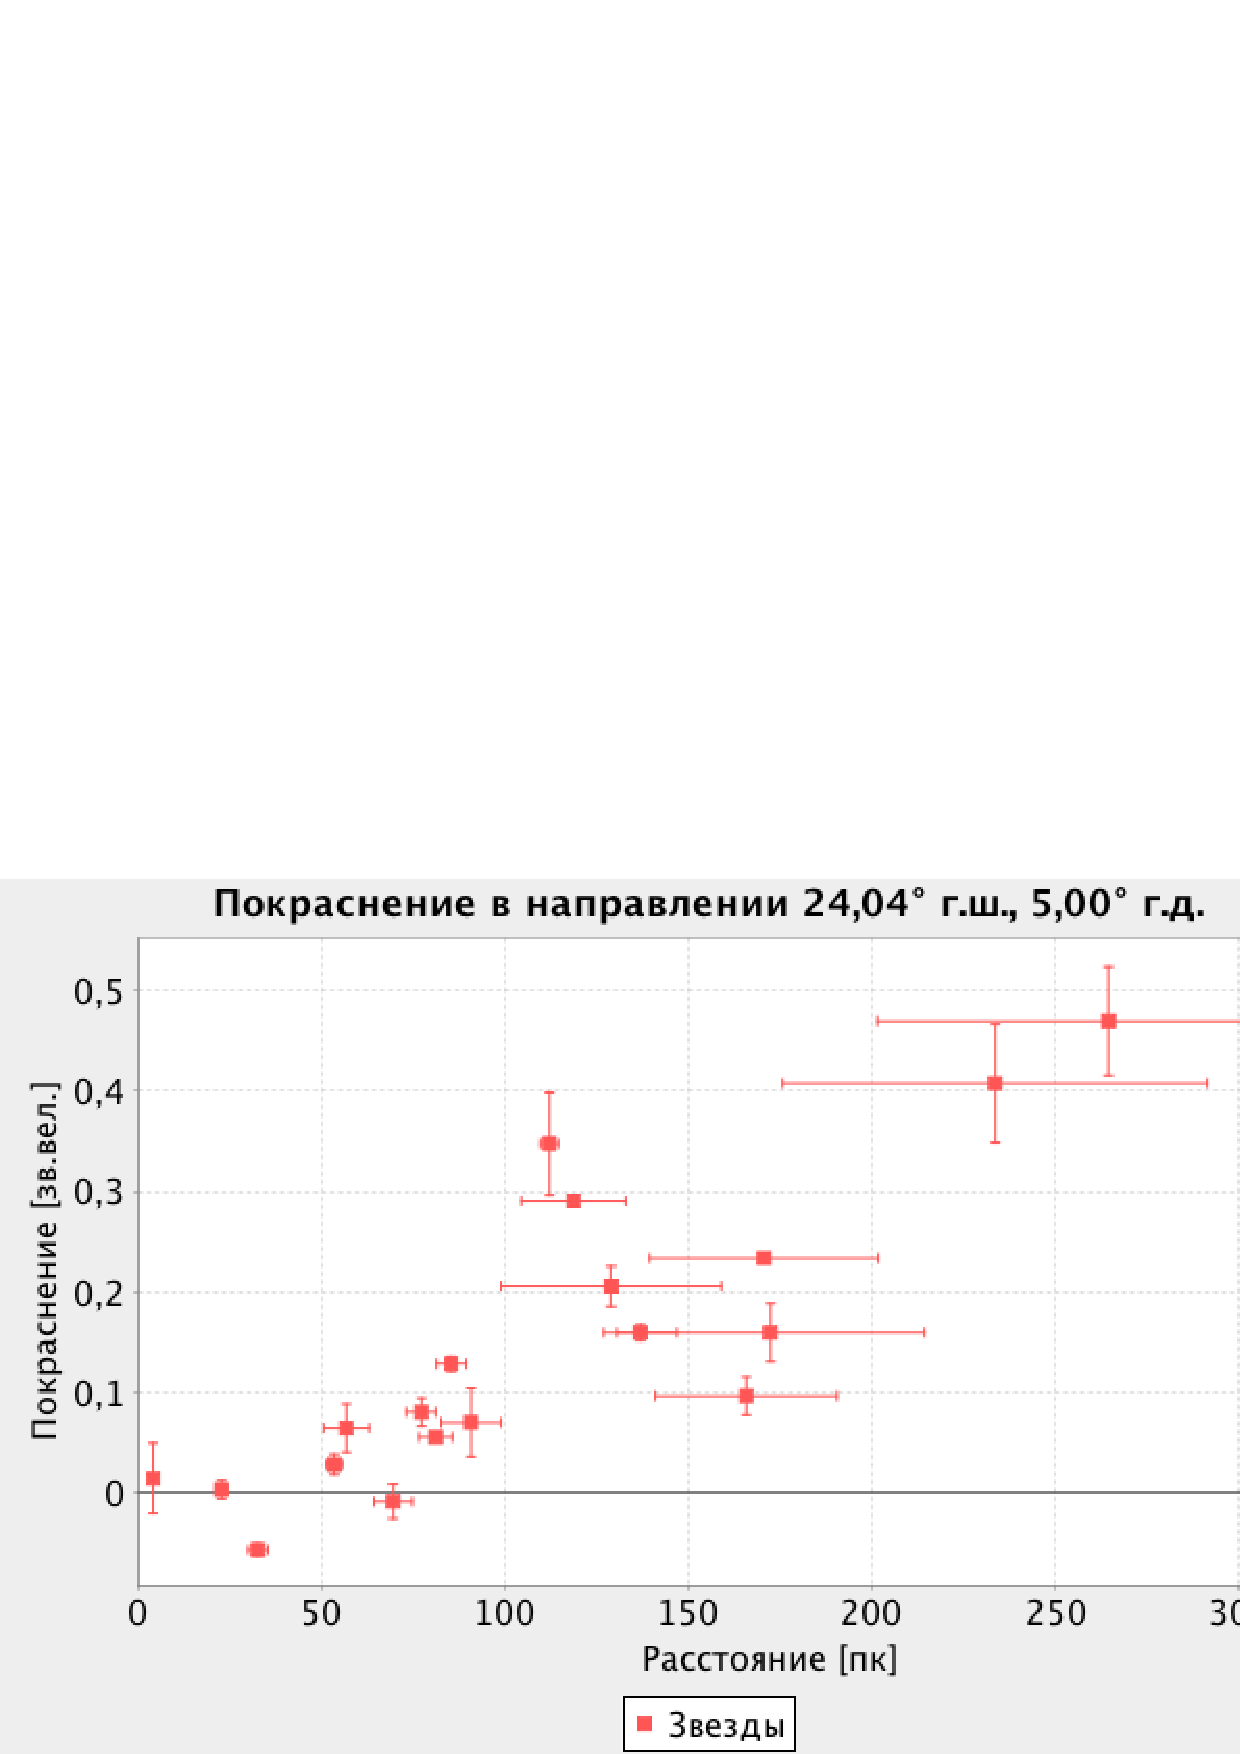
\includegraphics[scale=0.35]{real-1.png}
            \end{center}             
        \end{frame}
        
        \begin{frame}{Реальная <<кривая>> покраснения}
            \begin{center}
                \includegraphics[scale=0.35]{real-2.png}
            \end{center}             
        \end{frame}
        
        \begin{frame}{<<В среднем>>}
            \begin{center}
                \includegraphics[scale=0.35]{real-3.png}
            \end{center}             
        \end{frame}        
        
        \begin{frame}{Отрицательный тренд}
            \begin{center}
                \includegraphics[scale=0.35]{real-4.png}
            \end{center}             
        \end{frame}
        
    \section{Карты}            
        
        \begin{frame}{Коэффициент $a$ ~~~~~~~~~~~~~~~ $E = a r + b$}
            \begin{center}
                \includegraphics[scale=0.32]{map-a-white.png}
            \end{center}             
        \end{frame}
        
        \begin{frame}{Коэффициент $a$ с ошибкой}
            \begin{center}
                \includegraphics[scale=0.32]{map-a-sigma.png}
            \end{center}             
        \end{frame}
        
        \begin{frame}{Коэффициент $b$ ~~~~~~~~~~~~~~~ $E = a r + b$}
            \begin{center}
                \includegraphics[scale=0.32]{map-b-white.png}
            \end{center}             
        \end{frame}
        
        \begin{frame}{Коэффициент $k$ ~~~~~~~~~~~~~~~~~~~~~ $E = k r$}
            \begin{center}
                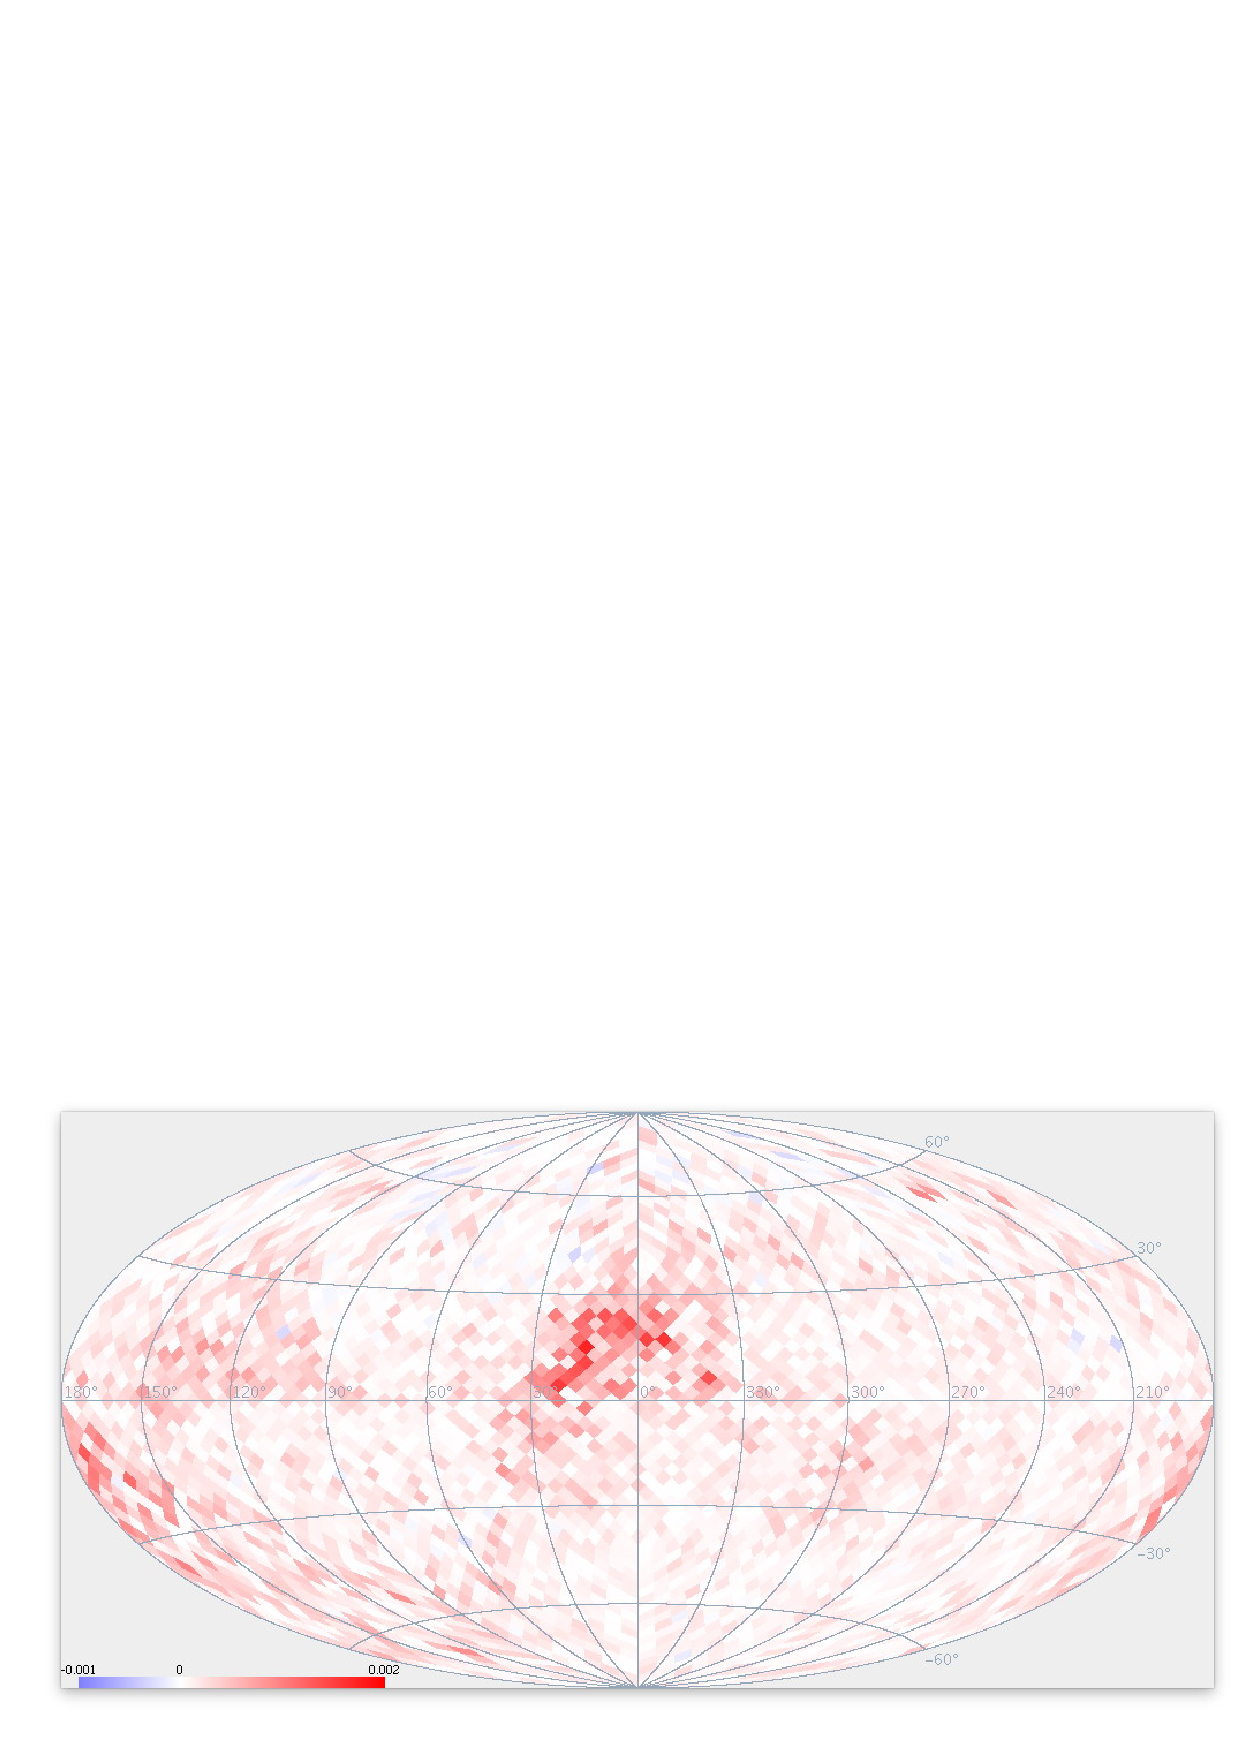
\includegraphics[scale=0.32]{map-k.png}
            \end{center}             
        \end{frame}
        
        \begin{frame}{Коэффициент $a$ ~~~~~~~~~~~~~~~ $E = a r + b$}
            \begin{center}
                \includegraphics[scale=0.32]{map-a-white.png}
            \end{center}             
        \end{frame}

    \section{Предварительная обработка}                
        
        \begin{frame}{Предварительная обработка}
            \begin{itemize}
                \item В расчет берутся 58486 из 118219 звезд
                \begin{itemize}
                    \item Отсутствие некоторых необходимых данных$^*$
                    \item Точность в расстоянии 25\%
                \end{itemize}
                \item Разбиение сферы на $12 \cdot 18^2 = 3888$ равновеликих частей алгоритмом Healpix
                \item Тренды строятся по 90\% расчетных звезд
                \item Расчет отсутствующих классов светимости
                \begin{itemize}
                    \item Спектральный класс, класс светимости $\Longrightarrow (B - V)_{int}$
                \end{itemize}
            \end{itemize}
        \end{frame}
        
        \begin{frame}{Наличие классов светимости}
            \begin{center}
                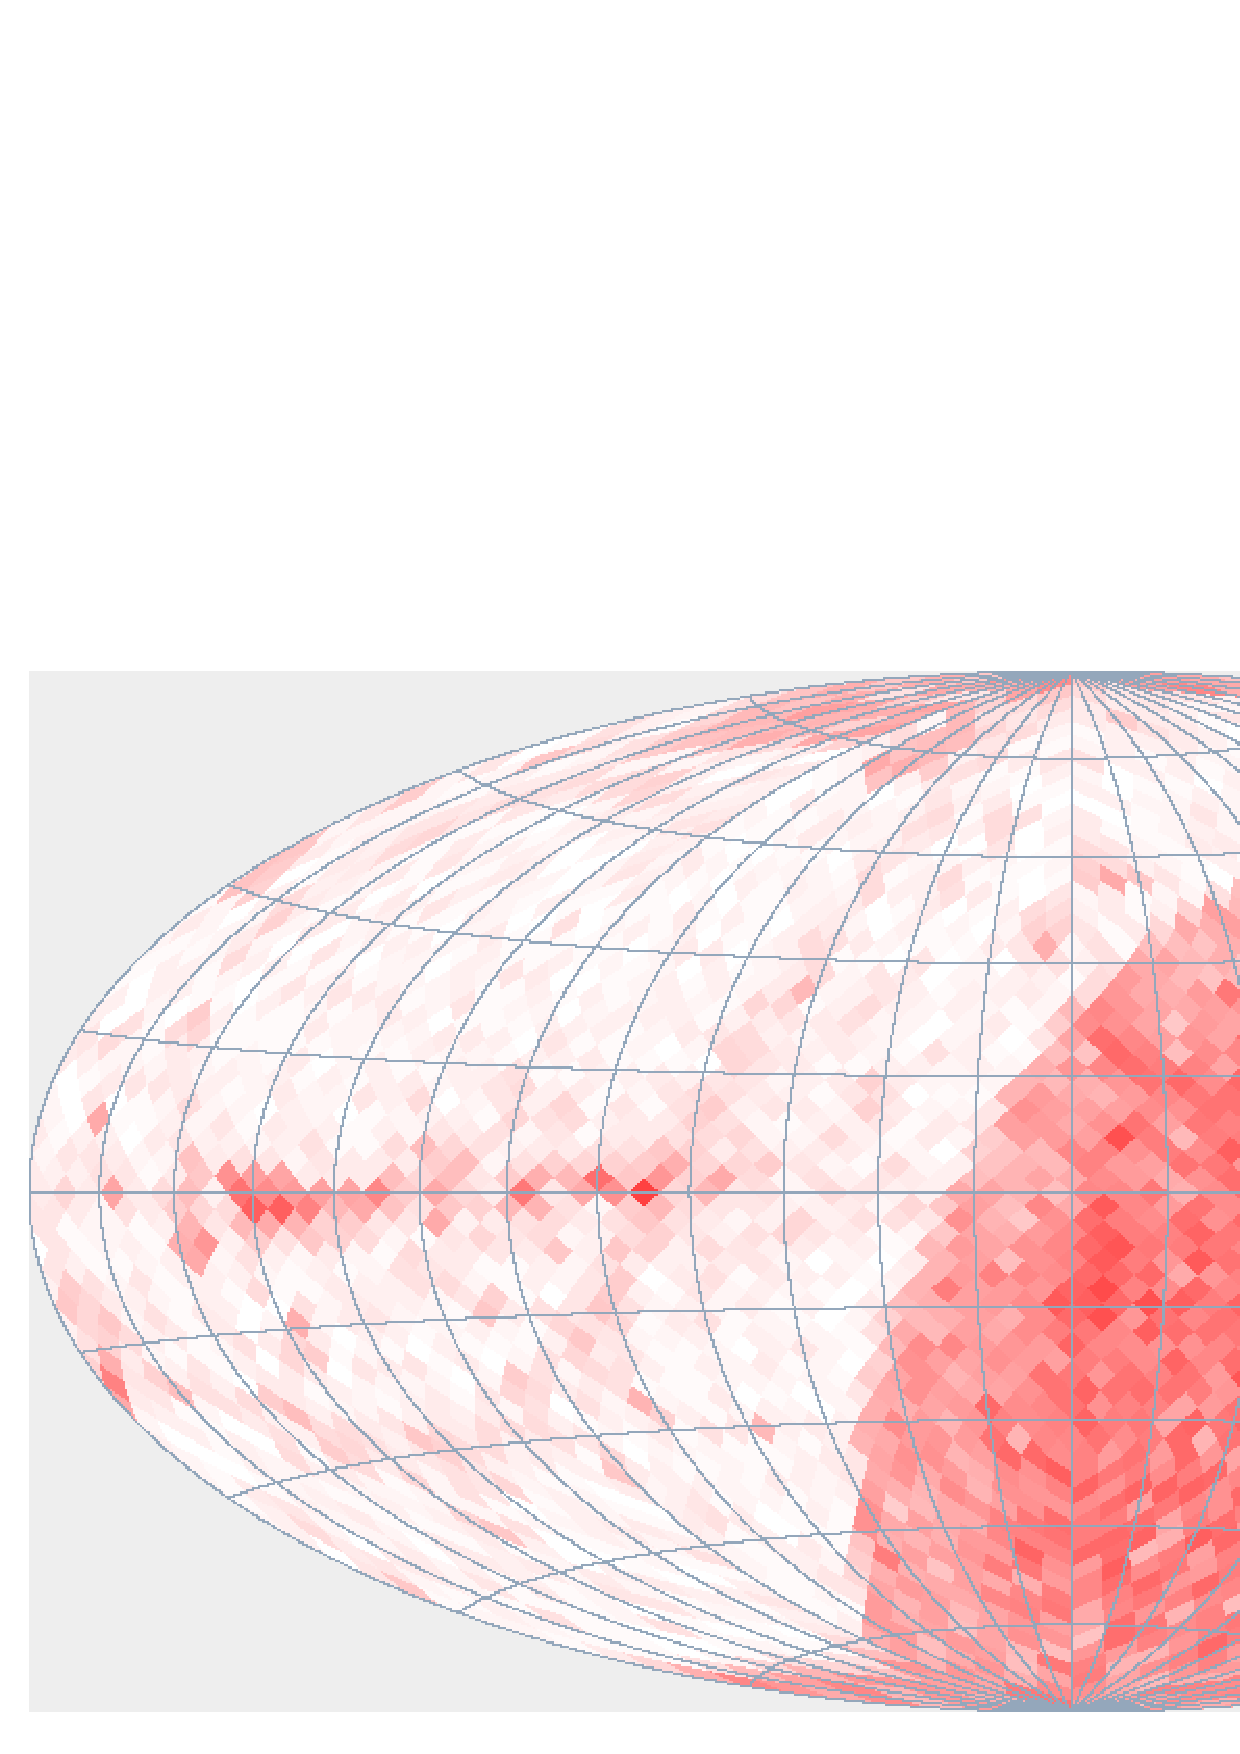
\includegraphics[scale=0.32]{count-white.png}
            \end{center}             
        \end{frame}

    \section{Определение классов светимости}                
        
        \begin{frame}{Обучение классификатора}
            \begin{itemize}
                \item Вспомним диаграмму Герцшпрунга--Рассела
                \item Факторы: показатель цвета, абсолютная звездная величина
                \item Класс: класс светимости
                \item Алгоритм классификации: метод опорных векторов (Support Vector Machines, SVM)
            \end{itemize}
        \end{frame}        
        
        \begin{frame}{Обучающее множество}
            \begin{center}
                \includegraphics[scale=0.25]{ml-1.png}
            \end{center}             
        \end{frame}
        
        \begin{frame}{Результат классификации}
            \begin{center}
                \includegraphics[scale=0.25]{ml-2.png}
            \end{center}             
        \end{frame}
        
        \begin{frame}{Качество классификации}
            Результаты кросс--валидации на 10 частях
            \begin{itemize}
                \item Точность 93.4\%
                \item Полнота 93.0\%
                \item F--мера 92.7\%
            \end{itemize}
            Замечание
            \begin{itemize}
                \item Обучение проводилось только на III и V классах
            \end{itemize}
        \end{frame}    

    \section{Результаты}                
        
        \begin{frame}{Результат}
            \begin{center}
                \includegraphics[scale=0.32]{map-a-white.png}
            \end{center}             
        \end{frame}
        
        \begin{frame}{Что дальше?}
            \begin{center}
                \includegraphics[scale=0.35]{next.png}
            \end{center}             
        \end{frame}    
        
        \begin{frame}{Q\&A}
            \begin{center}
                Спасибо за внимание!\\
                \href{https://github.com/amosov-f/DustDetection}{github.com/amosov-f/DustDetection}
                %{github.com/amosov-f/VorTree}
            \end{center}
        \end{frame}

\end{document}